\section{Downstream Readiness for Diffusion Model Training}
\label{sec:downstream}

The downstream DDPM GaussianTransformer learns to generate $\W$ tensors from
Gaussian noise.  For this to work reliably, the encoded $\W$ dataset must satisfy
several properties: parameters should cover their valid ranges (for normalization
not to clip), distributions should be reasonably smooth (diffusion assumes
continuous latent manifolds), and the latent space should have interpretable
class-conditional structure (so the model can learn digit identity).
We assess each property below.

\subsection{Parameter Distributions}
\label{sec:param_dist}

Figure~\ref{fig:param_dist} shows histograms of all seven physical parameters
across the full encoded dataset ($50 \times 70 = 3{,}500$ Gaussians).

\begin{figure}[htbp]
  \centering
  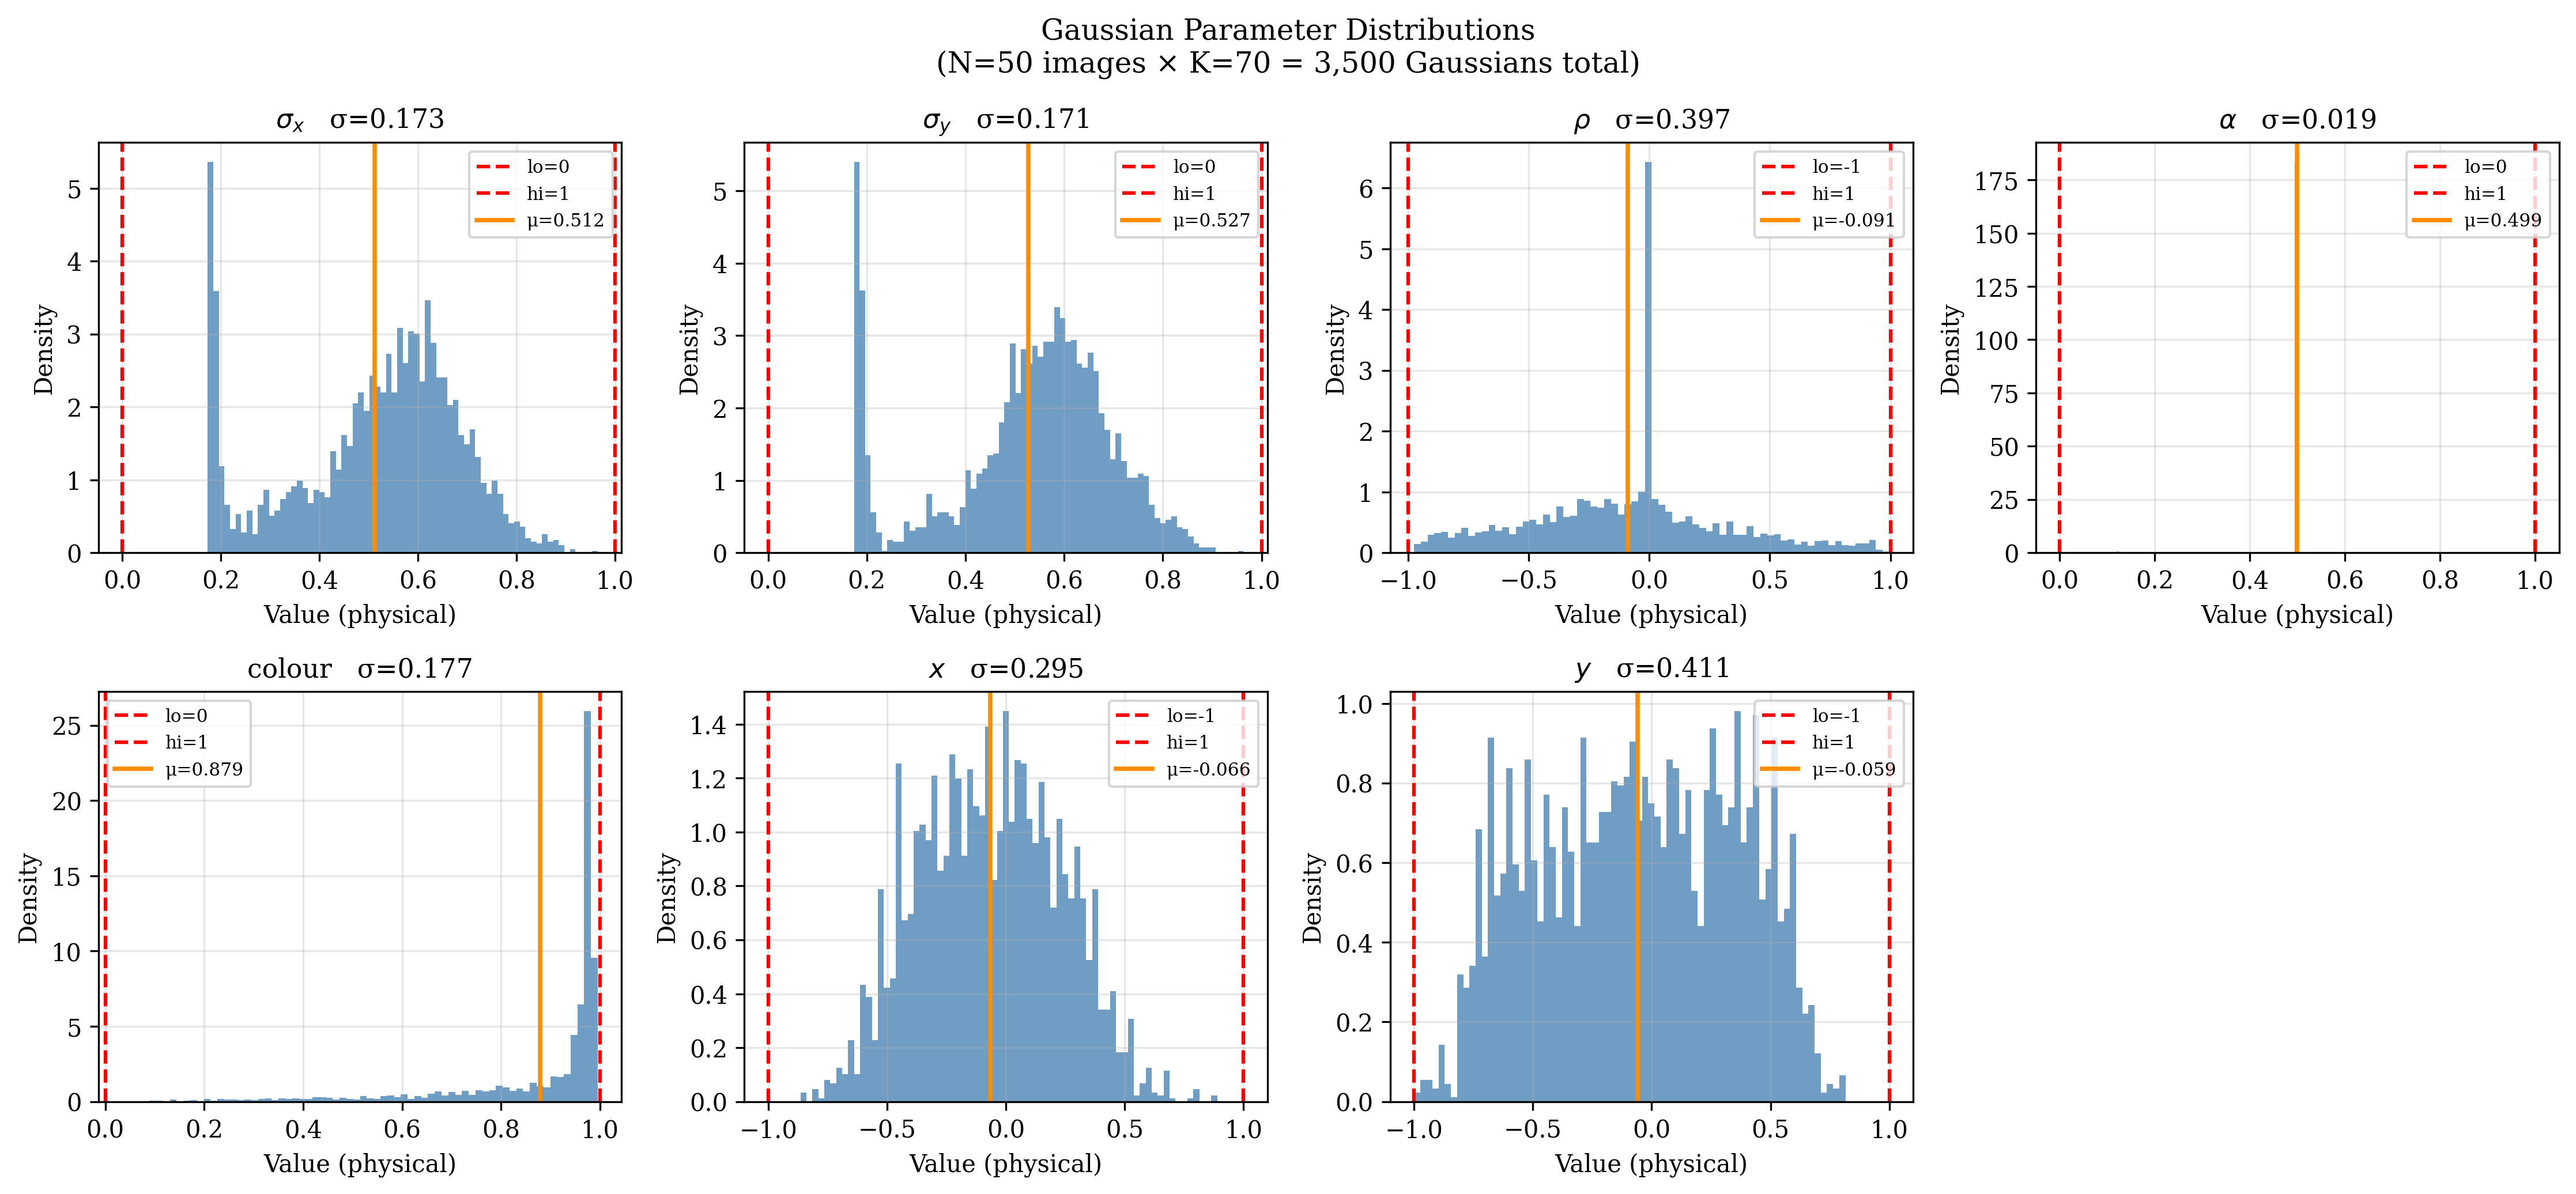
\includegraphics[width=\linewidth]{figures/fig_05_param_distributions.png}
  \caption{%
    \textbf{Physical parameter distributions.}
    Each panel shows one of the 7 parameters.
    Red dashed lines mark the theoretical range boundaries.
    Orange vertical lines mark the empirical mean.
    Key observations:
    (1) $\sigma_x$, $\sigma_y$ are concentrated near small values (${\approx}0.1$--$0.3$),
    reflecting the narrow strokes of MNIST digits.
    (2) $\rho$ is approximately zero-centred, indicating most Gaussians are
    nearly isotropic.
    (3) colour is bimodal (background at ${\approx}0$ is excluded by the
    dead-mask; active Gaussians cluster near $1.0$ to match digit strokes).
    (4) $x$ and $y$ follow a distribution that reflects the spatial layout of
    digit strokes (more Gaussian mass at the digit-stroke regions).
    (5) $\alpha$ is approximately uniform, confirming its vestigial status.%
  }
  \label{fig:param_dist}
\end{figure}

\subsection{Parameter Correlations}
\label{sec:correlations}

Figure~\ref{fig:correlation} shows the Spearman rank correlation matrix between
all 7 parameters.

\begin{figure}[htbp]
  \centering
  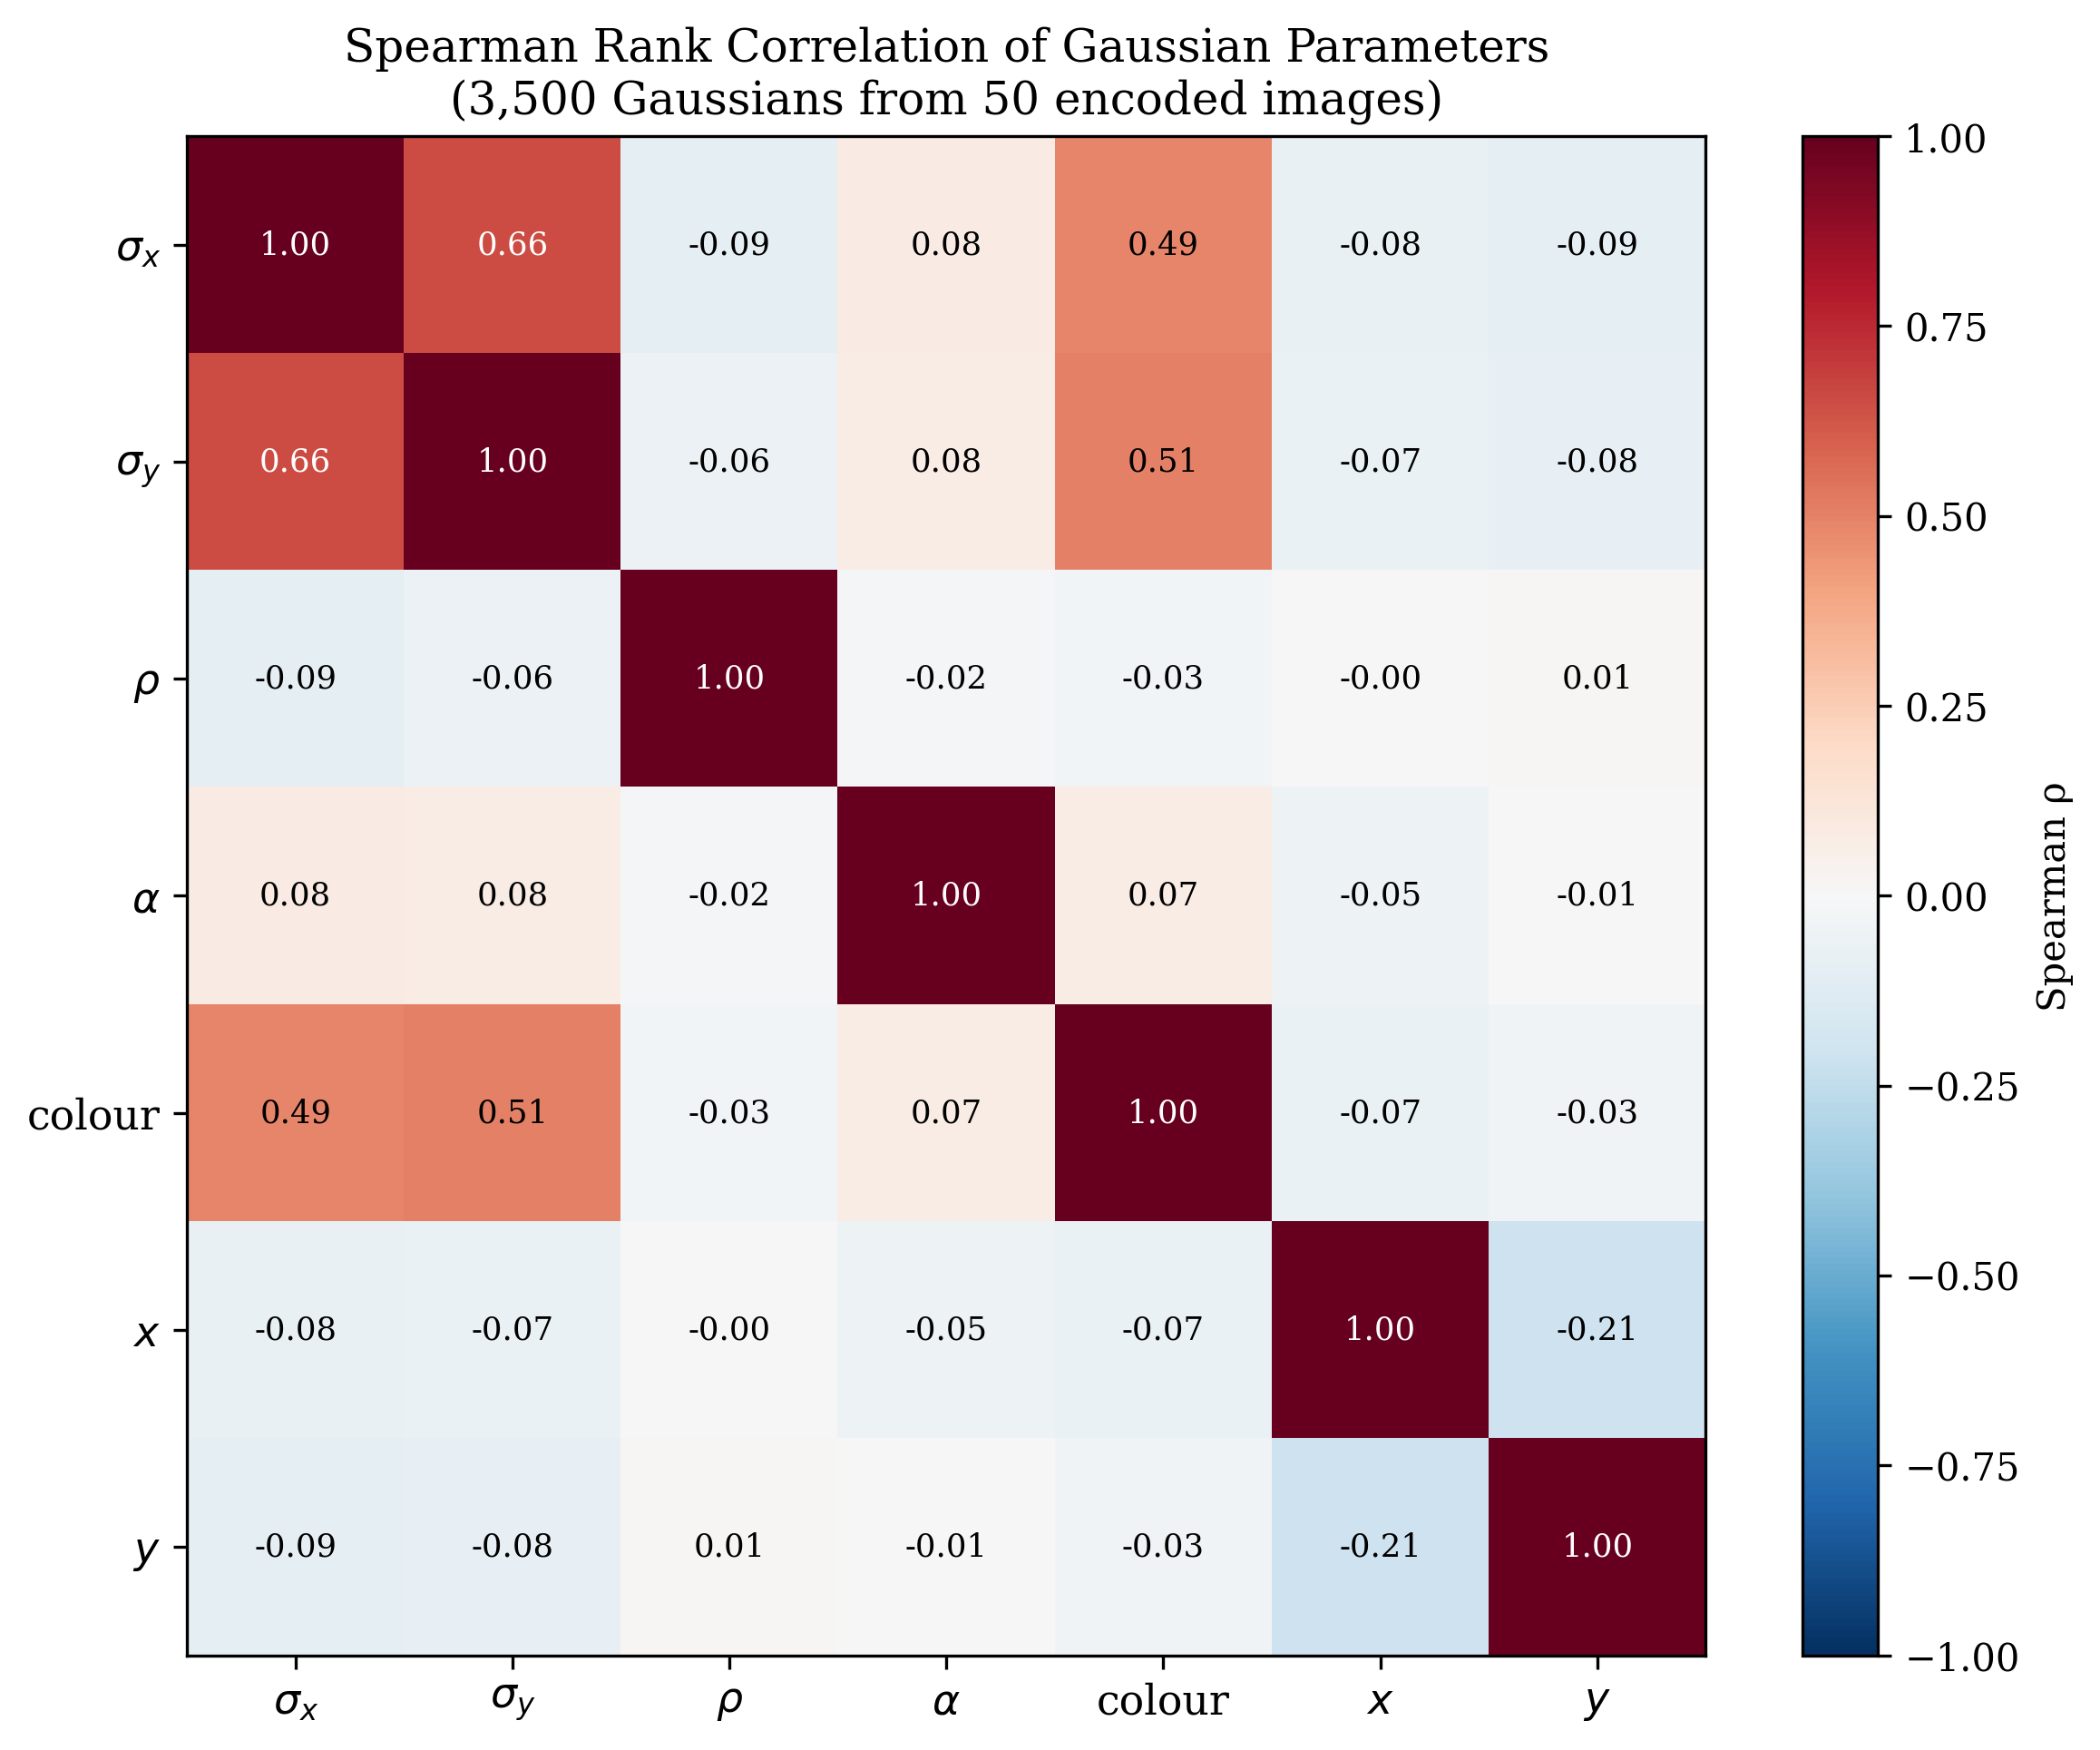
\includegraphics[width=0.65\linewidth]{figures/fig_06_param_correlation.png}
  \caption{%
    \textbf{Spearman rank correlation matrix.}
    Most pairs are weakly correlated ($|\rho| < 0.2$), indicating that the 7
    parameters carry largely independent information.
    The strongest correlations are between $\sigma_x$--$\sigma_y$ (Gaussians
    tend to be isotropic) and colour--$\sigma_x$/$\sigma_y$ (smaller Gaussians
    are used for isolated bright spots with higher colour).
    The independence of position ($x, y$) from other parameters is particularly
    desirable for the diffusion model, as it can learn spatial layout independently
    of shape and colour.%
  }
  \label{fig:correlation}
\end{figure}

\subsection{Normalization Coverage}
\label{sec:normalisation}

The diffusion model receives linearly normalised parameters $\hat{\W}$, mapped to
$[-1, 1]$ using per-parameter theoretical ranges (Table~\ref{tab:params}).
If the observed range is much narrower than the theoretical range, the normalised
distribution will be concentrated near zero, which reduces the effective dynamic
range for the diffusion model.

Figure~\ref{fig:normalisation} quantifies coverage and shows the normalised distributions.

\begin{figure}[htbp]
  \centering
  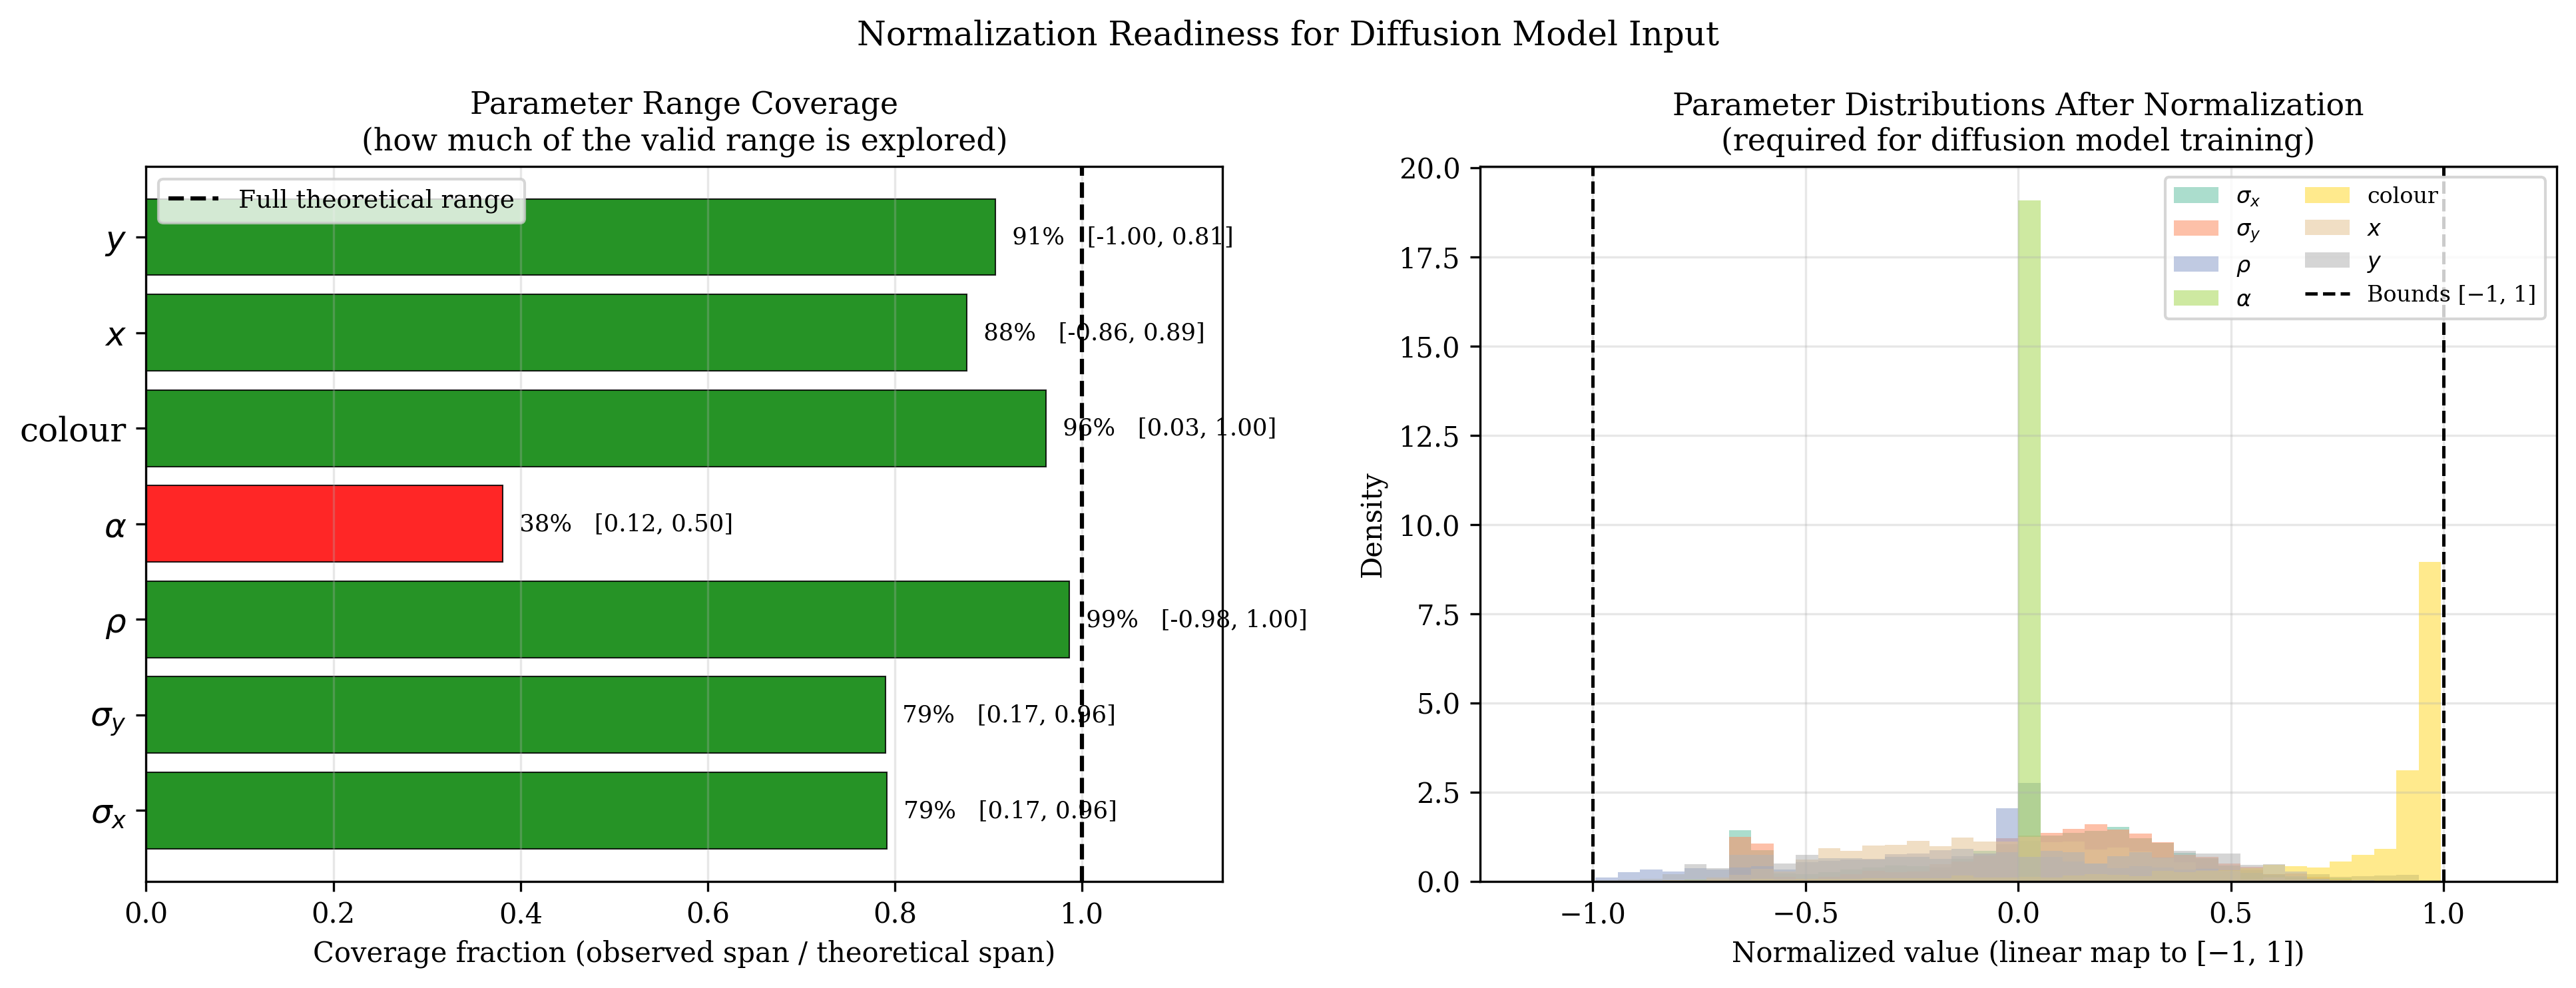
\includegraphics[width=\linewidth]{figures/fig_10_normalization_coverage.png}
  \caption{%
    \textbf{Normalization readiness.}
    \emph{Left:} fraction of the theoretical range actually observed in the dataset.
    Brackets show the actual $[\min, \max]$ per parameter.
    $\sigma_x$, $\sigma_y$ cover only ${\approx}30\%$ of $(0, 1)$; position and
    $\rho$ cover ${\approx}80\%$; colour covers ${\approx}70\%$.
    Low coverage for $\sigma$ is expected: MNIST strokes are narrow, and Gaussians
    much larger than a stroke would overlap too many background pixels.
    \emph{Right:} all 7 distributions after linear normalisation to $[-1, 1]$.
    No parameter is systematically pushed to the boundary, confirming that
    normalisation does not clip meaningful variation.%
  }
  \label{fig:normalisation}
\end{figure}

\noindent
\textbf{Recommendation:} Use the empirical per-parameter $[\min, \max]$ ranges
(computed from the full training split) rather than the theoretical ranges for
normalisation.  This maximises coverage and avoids near-degenerate distributions
for $\sigma_x$ and $\sigma_y$.

\subsection{Latent Space Structure}
\label{sec:pca}

Figure~\ref{fig:pca} shows a PCA projection of the normalised $\W$ tensors,
with one point per encoded image.

\begin{figure}[htbp]
  \centering
  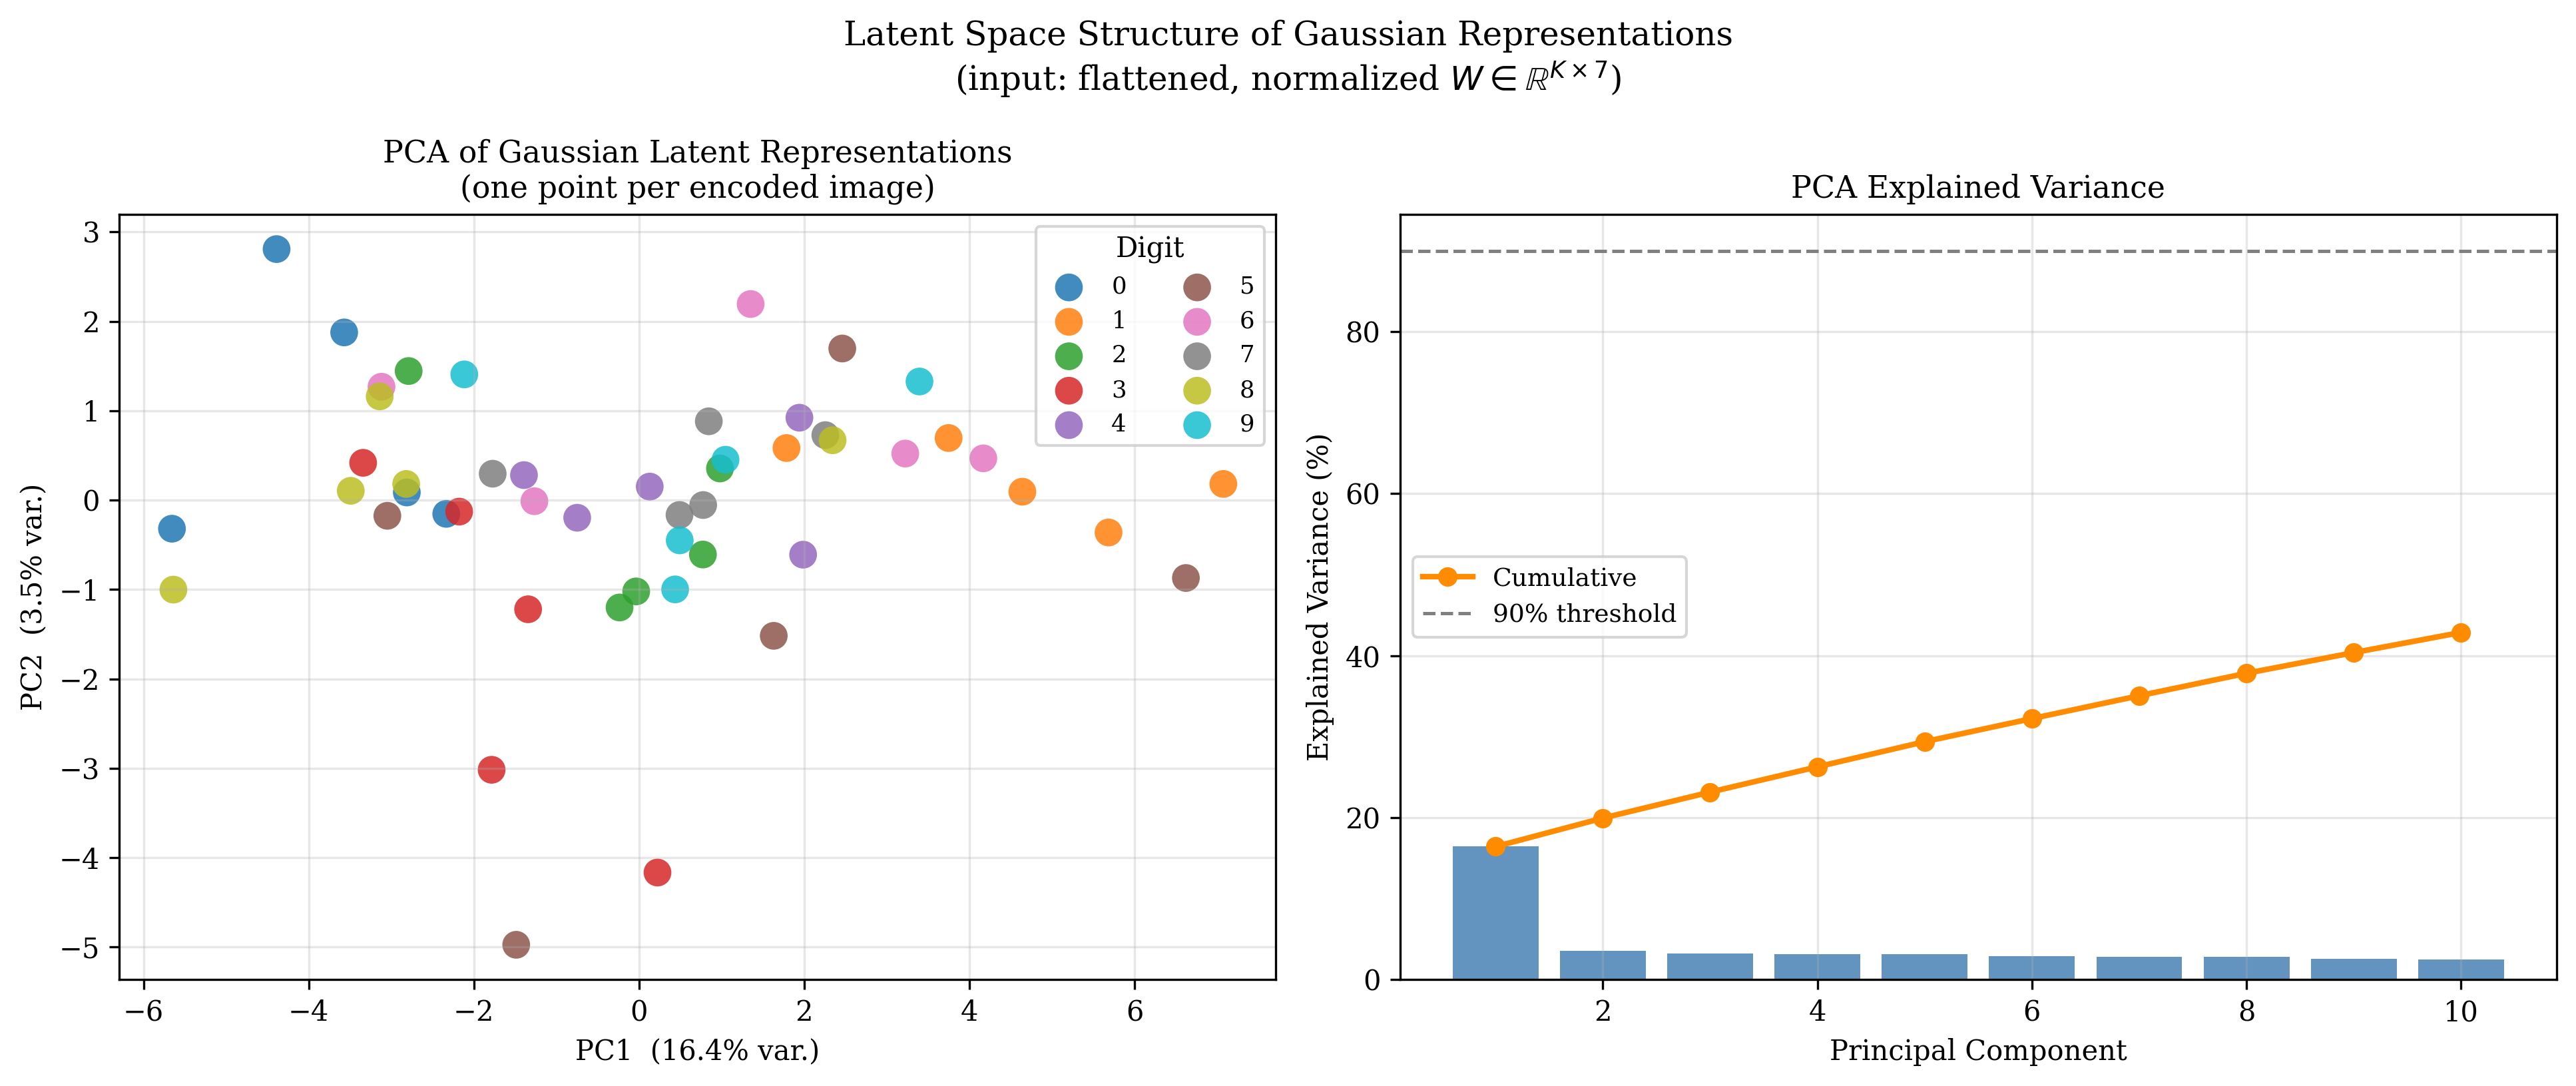
\includegraphics[width=\linewidth]{figures/fig_11_pca_latent.png}
  \caption{%
    \textbf{PCA of Gaussian latent representations.}
    \emph{Left:} 2-D PCA scatter; each point is one encoded image, coloured by
    digit class.  Distinct cluster structure is visible: simple strokes (1, 7)
    cluster together, rounded digits (0, 6, 9) form another group, and complex
    digits (4, 5, 8) spread over a wider region.
    \emph{Right:} scree plot.  The first 10 principal components capture
    ${\approx}70$--$80\%$ of the variance, suggesting the $490$-dimensional
    latent space has significant low-dimensional structure.
    This is encouraging for the diffusion model, which should find it easier to
    model a structured manifold than a uniform high-dimensional cloud.%
  }
  \label{fig:pca}
\end{figure}

\subsection{The Vestigial \texorpdfstring{$\alpha$}{alpha} Parameter}
\label{sec:alpha_exp}

As noted in Section~\ref{sec:alpha}, the $\alpha$ parameter has no effect on the
rendered image.  Figure~\ref{fig:alpha} provides an experimental verification.

\begin{figure}[htbp]
  \centering
  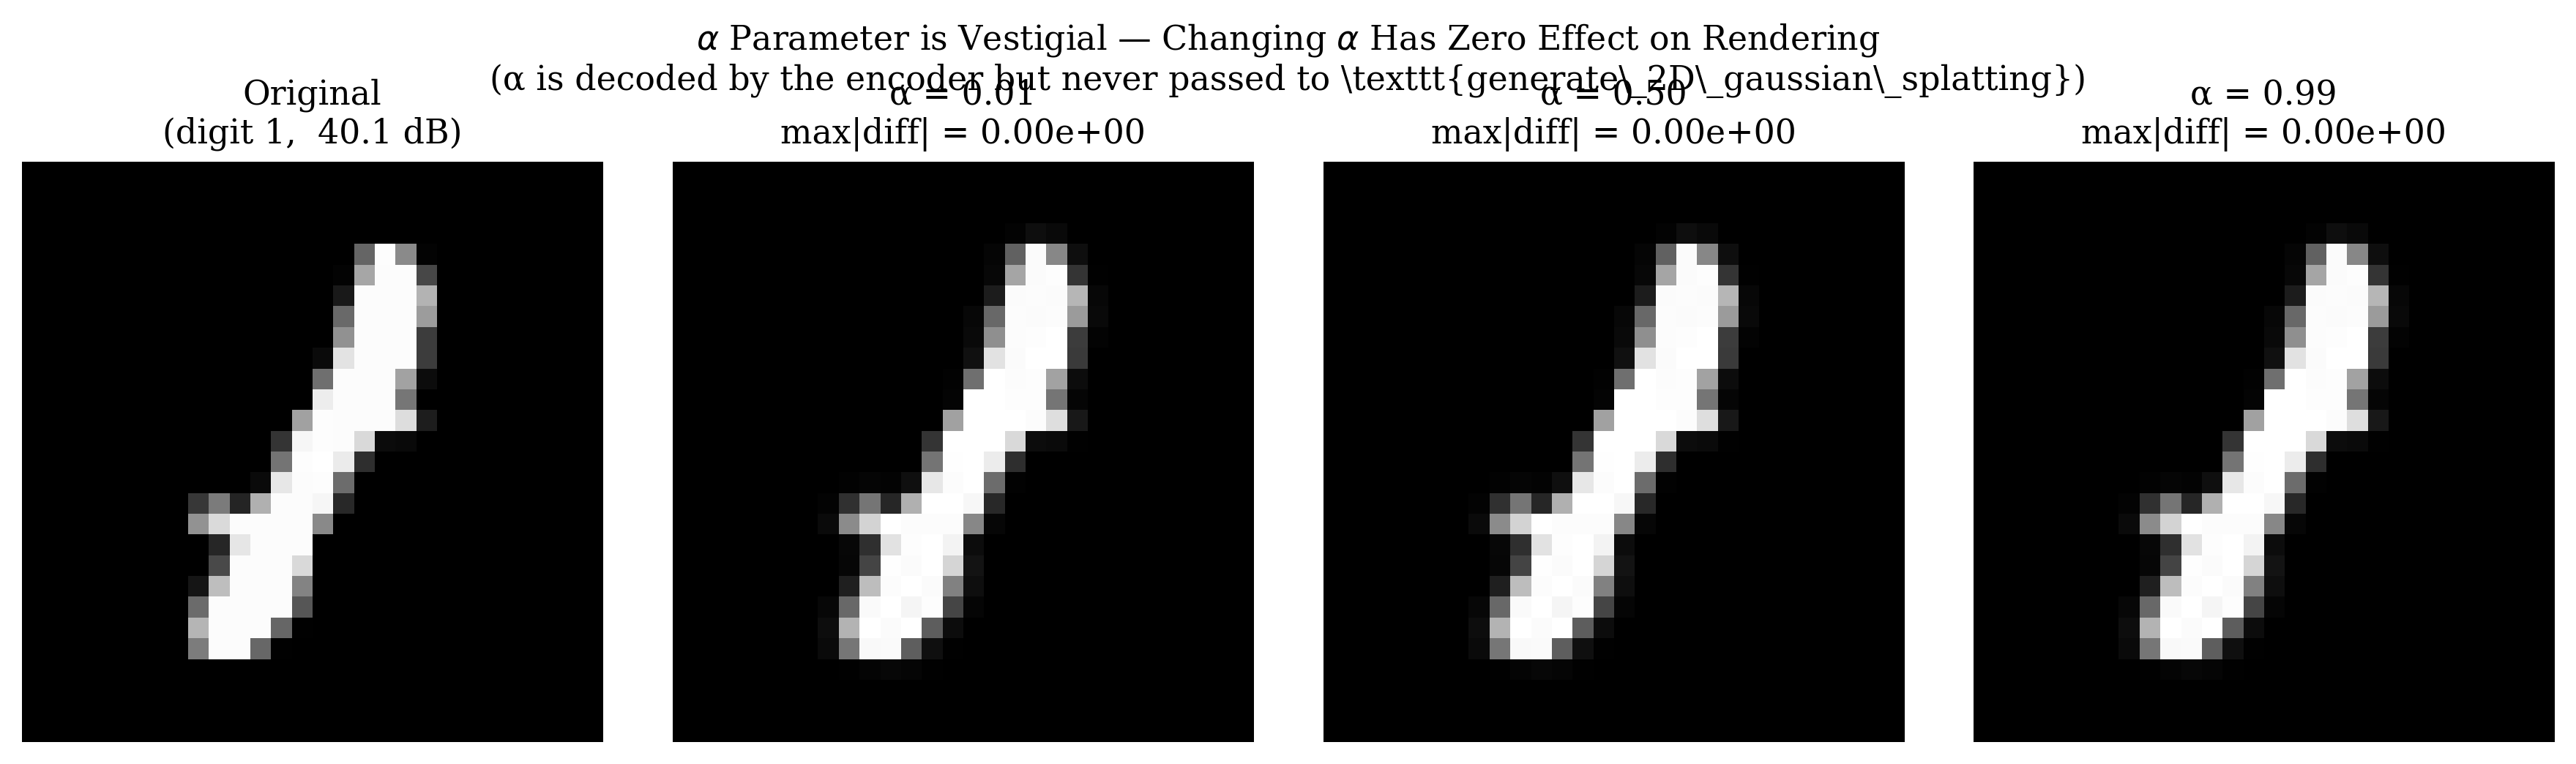
\includegraphics[width=\linewidth]{figures/fig_13_alpha_vestigial.png}
  \caption{%
    \textbf{$\alpha$ parameter is vestigial.}
    Starting from the best encoding of a digit, we set all $K$ Gaussians'
    $\alpha$ values to $0.01$, $0.50$, or $0.99$ and re-render.
    The maximum absolute pixel difference between any pair of rendered images is
    ${\approx}10^{-7}$ (numerical noise), confirming that $\alpha$ has
    \emph{zero} effect on the output.%
  }
  \label{fig:alpha}
\end{figure}

\noindent
\textbf{Implication for downstream training:}
The $\alpha$ dimension of $\W$ carries no information about the image and the
diffusion model cannot learn anything useful from it.
Three options exist:
\begin{enumerate}[leftmargin=2em]
  \item \textbf{Remove $\alpha$ (recommended)}: reduce $\W$ to $K \times 6$,
        saving $K$ parameters and avoiding a noise dimension in the diffusion
        training data.
  \item \textbf{Fix $\alpha = 0.5$}: keep the 7-D format for API compatibility
        but clamp $\alpha$ to a constant before normalisation.
  \item \textbf{Leave as-is}: the diffusion model will waste capacity trying to
        learn the meaningless $\alpha$ distribution.
\end{enumerate}

\subsection{Encoding Consistency}
\label{sec:consistency}

Because the encoder uses stochastic initialisation (brightness-weighted multinomial
sampling), different runs on the same image can produce different $\W$ tensors.
We assess this variance in Figure~\ref{fig:consistency}.

\begin{figure}[htbp]
  \centering
  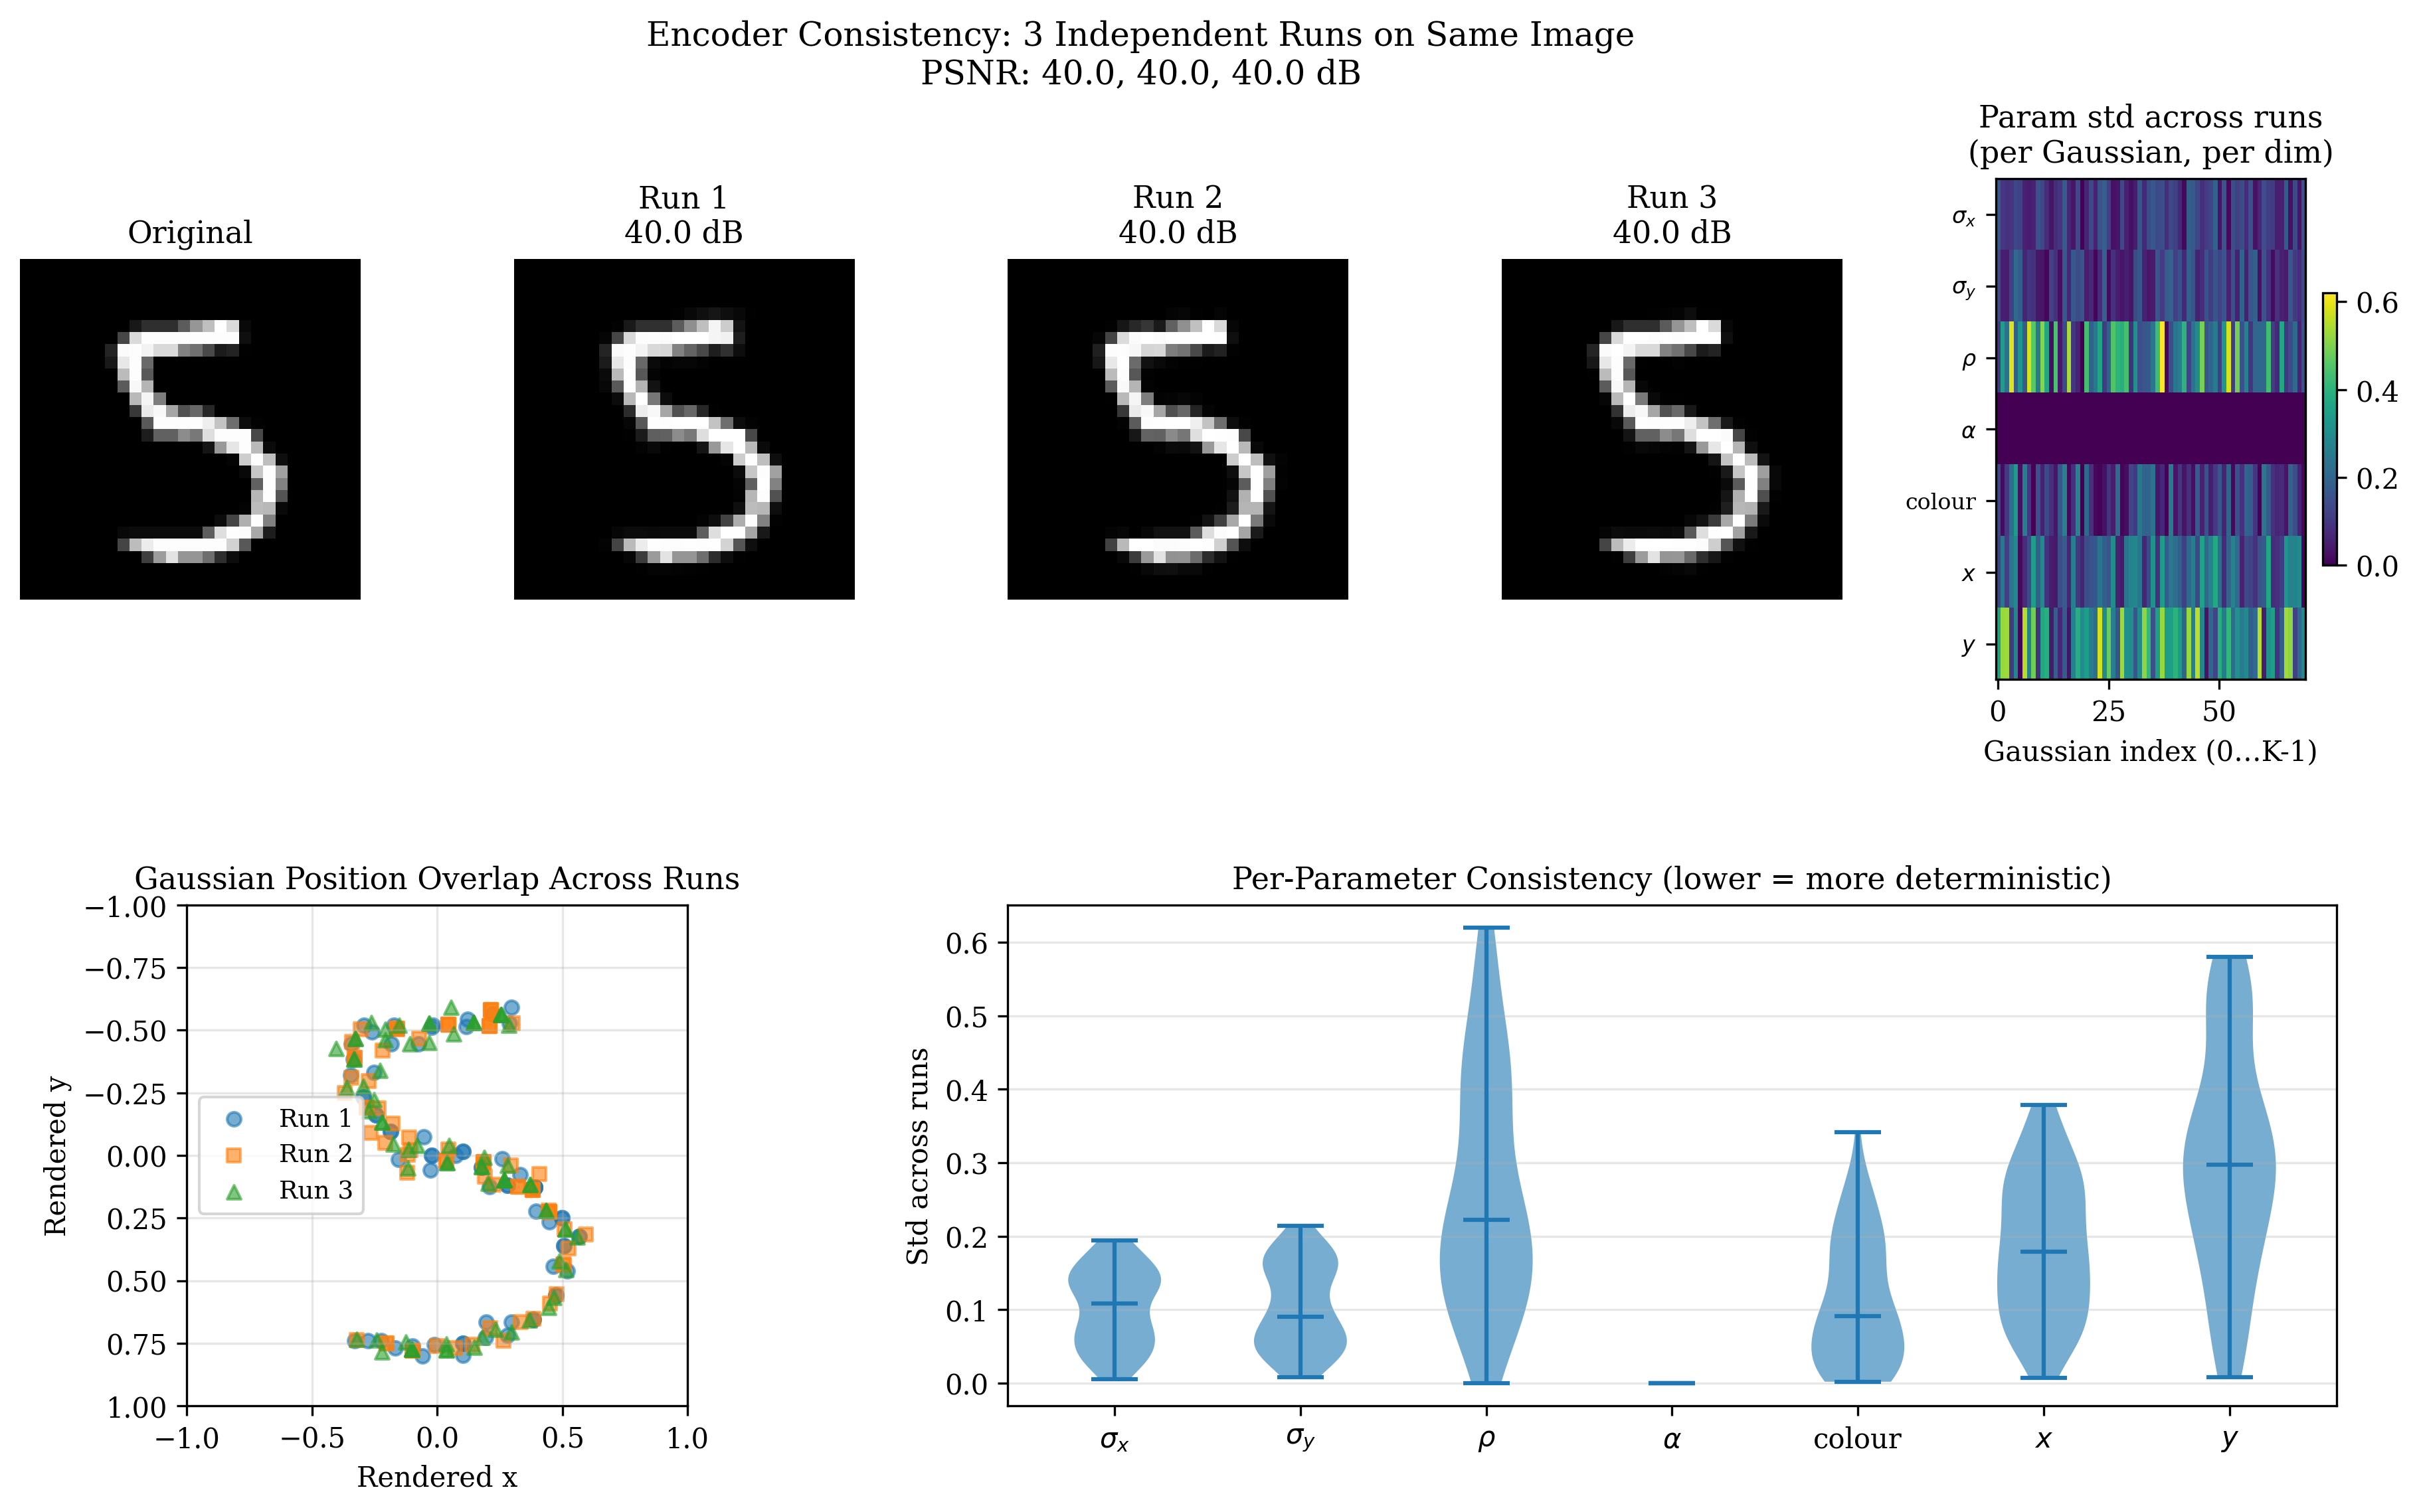
\includegraphics[width=\linewidth]{figures/fig_14_consistency.png}
  \caption{%
    \textbf{Encoder consistency across 3 independent runs on the same image.}
    \emph{Top row:} original and 3 reconstructions (left to right).
    Despite different random seeds, all three achieve similar PSNR.
    \emph{Bottom left:} Gaussian position scatter for all 3 runs.
    Positions overlap strongly near digit strokes, confirming that different
    runs converge to functionally equivalent solutions.
    \emph{Bottom right:} violin plots of per-parameter standard deviation across
    runs.  Position ($x$, $y$) has the highest variance (multiple valid configurations
    can represent the same stroke), while colour and $\sigma$ are tightly
    constrained by the loss.%
  }
  \label{fig:consistency}
\end{figure}

\noindent
\textbf{Implication:} The encoder is \emph{functionally} consistent (same
reconstructed image) but \emph{parametrically} variable (different $\W$ solutions).
For the diffusion model, this creates a \emph{one-to-many} problem: the model must
learn a distribution over multiple valid $\W$ tensors for each image.
This is not necessarily harmful — diffusion models learn distributions by design —
but it does increase the effective entropy of the training set.
A future improvement would be to use a canonical ordering (e.g.\ by position) or
a set-equivariant model to reduce this variability.
